\documentclass[runningheads,a4paper]{llncs}
\usepackage{amssymb}
\setcounter{tocdepth}{3}
\usepackage{listings}
\usepackage{booktabs}
\usepackage{mathtools}
\usepackage{tabularx}
\usepackage{fixltx2e}
\PassOptionsToPackage{hyphens}{url}\usepackage{hyperref}
\usepackage[hyphens]{url}
\usepackage{upquote,textcomp}
\lstset{breaklines=true, basicstyle=\scriptsize\ttfamily, upquote=true}

\usepackage{fancyvrb}
\VerbatimFootnotes
\usepackage{cprotect}

\usepackage{graphicx}
\makeatletter
\def\maxwidth#1{\ifdim\Gin@nat@width>#1 #1\else\Gin@nat@width\fi}
\makeatother

\usepackage{amsmath}
\usepackage{pmml-new}

\usepackage{color,graphics,array,csscolor}

\usepackage{fontspec,unicode-math}
\usepackage[Latin,Greek]{ucharclasses}
\setTransitionsForGreek{\fontspec{Times New Roman}}{}

\usepackage{subscript}
\lstset{breaklines=true, basicstyle=\scriptsize\ttfamily}

\begin{document}
\mainmatter

\title{Ontology-driven Visual Exploration of Preclinical Research Data in the Spinal Cord Injury Domain}
\titlerunning{Ontology}
\author{Alexander Borowi\inst{1} \and
Hendrik ter Horst\inst{1} \and
Matthias Hartung\inst{1} \and
Veronica Estrada\inst{2} \and
Nicole Brazda\inst{2} \and
Hans Werner Müller\inst{2} \and
Philipp Cimiano\inst{1}}
\authorrunning{Alexander Borowi et al.}
\institute{CITEC, Bielefeld University, Germany\and
Neurology, HHU Düsseldorf, Germany\\
\email{aborowi@techfak.uni-bielefeld.de, 
hterhors@cit-ec.uni-bielefeld.de, 
mhartung@cit-ec.uni-bielefeld.de, 
veronica.estrada@uni-duesseldorf.de, 
nicole.brazda@uni-duesseldorf.de, 
hanswerner.mueller@uni-duesseldorf.de, 
cimiano@cit-ec.uni-bielefeld.de}}
\maketitle

\begin{abstract}
We present SCIExplorer\footnote{\url{http://psink.techfak.uni-bielefeld.de/SCIOExplorerv2/index.xhtml}}, an interactive web application for browsing research data represented in RDF format. Offering an intuitive exploration of the data in a visual interface based on the data-describing ontology, SCIExplorer is designed to overcome the potentially high entrance barriers faced by human domain experts interested in investigating research results at a glance without the need to formulate complex queries. In contrast, SCIExplorer provides filter-driven dynamic generation of SPARQL queries without the need to specify them manually. We demonstrate that the tool can be effectively used to answer relevant competency questions in the domain of spinal cord injury, thus providing intuitive access to the results of preclinical studies which are represented in RDF. In particular, SCIExplorer offers drill-downs to individual preclinical results in order to visualize their core parameters at an interpretable level of abstraction that is guided by an underlying domain ontology.

\keywords{Linked Data, Ontology-based Access, Open Research Data, Spinal Cord Injury, Visual Data Analytics}
\end{abstract}


\section{Introduction}

The amount of openly available research data in machine-readable formats such as RDF is constantly growing, due to the rise of open research portals, on the one hand, and successively more powerful natural language processing tools offering the capability of transforming unstructured data into structured form, on the other. Being tailored to automated processing by machines and services, these data sources are often hard to access by human researchers, as research data in various domains are inherently highly complex, and the data representation formalisms impose high barriers to human domain experts regarding their ability to interact with the data source. Against this background, the need for low-level, intuitive access to research data in RDF or derived formalisms becomes more important than ever. Current approaches towards browsing linked data such as LODmilla  \cite{__RefNumPara__9808_1959585331}, Yuzu  \cite{__RefNumPara__9846_1959585331}, Disco  \cite{__RefNumPara__9848_1959585331} or Tabulator  \cite{__RefNumPara__9850_1959585331} closely follow the RDF data model. In case of complex knowledge structures as they are ubiquitous in research data, this may result in obfuscation due to a multitude of triples which need to be browsed.

In this work, we present SCIExplorer, an interactive web application for investigating the results of preclinical studies in the spinal cord injury (SCI) domain that are represented in RDF. Offering an intuitive exploration of the data in a visual interface based on the data-describing ontology, SCIExplorer is designed to overcome the aforementioned problems, thus enabling domain experts without profound technical knowledge to formulate complex queries that are meaningful from a research perspective. In particular, the tool provides filter-driven dynamic generation of SPARQL queries without the need to specify them manually, and offers drill-downs to individual preclinical results in order to visualize their results and core parameters at a glance. We demonstrate that SCIExplorer can be effectively used to answer relevant domain-specific competency questions provided by experts.

\section{Background: Automatically Populating a Spinal Cord Injury Knowledge Base from Preclinical Studies}

Our motivation to develop an exploration tool for efficiently browsing RDF research data arose in the context of the PSINK project\footnote{\url{http://www.psink.de}}, that aims at ontology-based information extraction from large amounts of preclinical studies in the SCI domain. The main project goal is to create the first comprehensive SCI knowledge base in order to foster translation from preclinicial research into therapeutic concepts that are likely to be effective in human patients. The resulting knowledge structures, i.e., the results of preclinical studies, are represented in an RDF database that can be queried via SPARQL. Both the information extraction process and the data representation scheme underlying the SCIExplorer are guided by the Spinal Cord Injury Ontology (SCIO) that is specifically developed in this project  \cite{__RefNumPara__9937_1959585331}. Currently, SCIO contains over 500 entities and relations describing a preclinical study in a very fine-grained and well-structured way.

\section{SCIExplorer}

This tool was developed to explore the complex structures of preclinical studies that follow the conceptualization provided by the Spinal Cord Injury Ontology. The interface is generated semi-automatically given the specifications of an ontology and a configuration file. The latter is used to enable different views to the data, thus focusing on different aspects of SCIO.

{\bf Technical Details. }SCIExplorer is a stand-alone framework written in Java, HTML and PHP.\footnote{\url{https://github.com/ag-sc/SCIExplorer}} It is accessible though common web-browsers. The graphical interfaces relies on the JavaEE standard JavaServer Faces -- Framework (JSF) that is based on Servlets and JavaServer Pages (JSP). The content management is realized with PrimeFaces. 

{\bf System Architecture. }Fig.~\ref{refFigure0} shows the overall system architecture. This work focuses on the SCIExplorer (grey box) that is divided into three main parts:
\begin{figure}[h!]
\centering
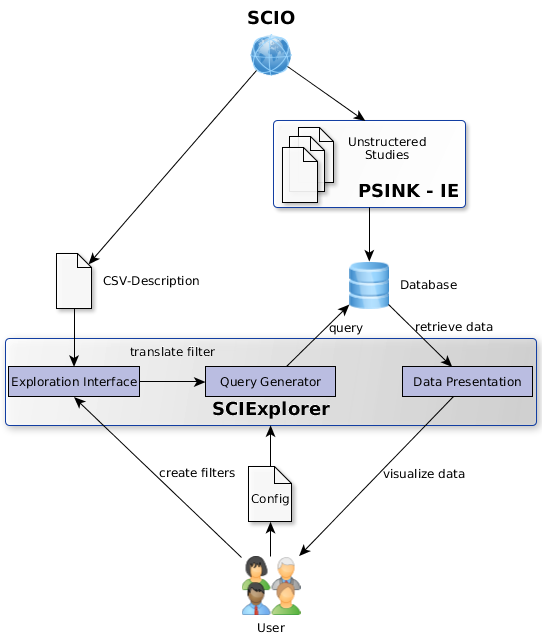
\includegraphics[width=\maxwidth{\textwidth}]{img/100002010000021E00000282A9ECCEA52E89BA7E.png}
\cprotect\caption{System Architecture}
\label{refFigure0}
\end{figure}

\begin{enumerate}
\item The {\em Exploration Interface} serves as an entry point. It is aligned to the ontology and modified by a configuration file that specifies different views to the data. The data exploration is driven by various filter strategies that are automatically extracted from the ontology.
\item The {\em Query Generator} automatically transforms set filters (based on concepts and properties provided by SCIO) into SPARQL statements.
\item The extracted data is prepared and visualized in the {\em Data Presentation} module. The configuration file specifies the parts of the data that should be viewed. 
\end{enumerate}

In the following, all parts a